\subsection{Class Diagram}

The architecture of our webapp is based on four principal items:
\begin{itemize}
    \item Resource
    \item Dao
    \item Servlet
    \item Filter
\end{itemize}

\subsection*{Resource}

In the figure \ref{fig:ResouceClassDiagram} it is possible to observe the 
architecture of the resources, that all implement the Resource interface 
that contains the \texttt{toJSON()} method. 
The reason for which it has been realized an interface and not an abstract 
class is because of the greater possibilities that offers an interface in 
java, in particular an enumeration can implement an interface, it cannot 
extend an abstract class, this allows us to manage also the enumerations 
as resources.

It has been used the \texttt{org.json} package also used by the tutor, in the 
use is more  immediate and requires less code overhead than 
\texttt{fasterxml.jackson} package.


\begin{figure}[H]
    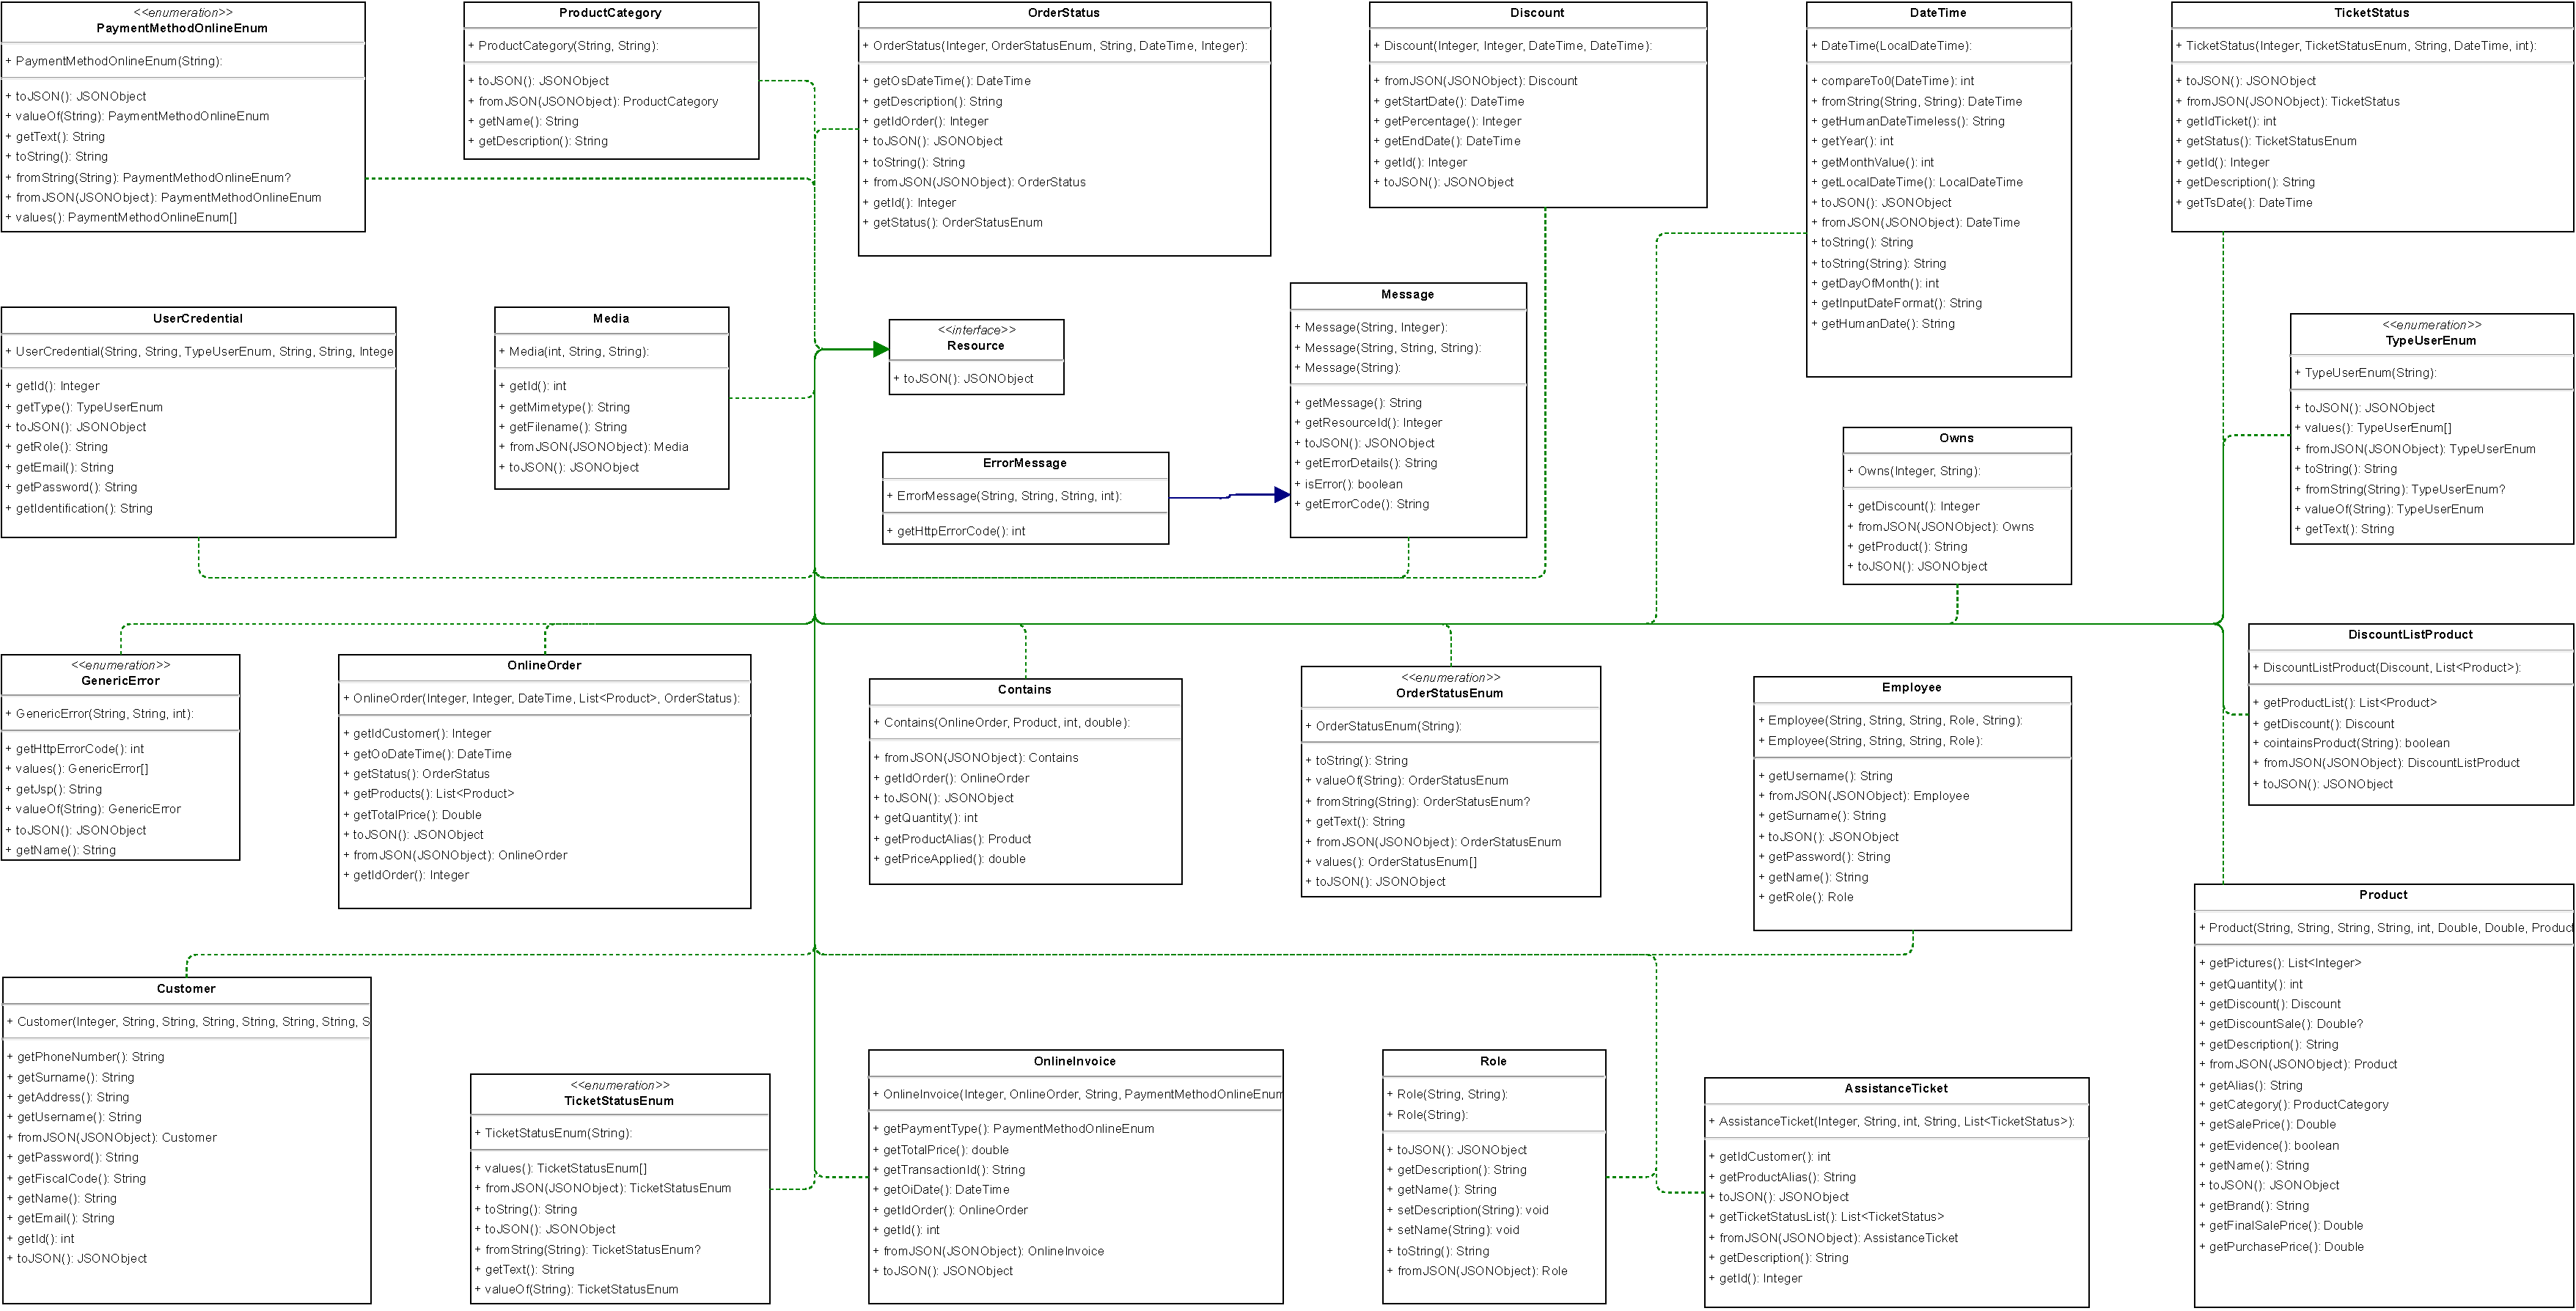
\includegraphics[width=\textwidth,height=\textheight,keepaspectratio]{Schemas/resources.drawio.pdf}
    \caption{Resource class diagram}
    \label{fig:ResouceClassDiagram}
\end{figure}

\subsection*{Dao}

Since daos have no inheritance (there 
is no basic dao), we do not include the dao schema.
Regardless they are already divided into subpackages for the table they 
operate on, although they are an important part of the project.


\subsection*{Servlet}

In the figure \ref{fig:ServletClassDiagram} it is possible to observe the 
architecture of the servlet. 
We defined this structure in order to maintain a functional separation 
between the web pages and the ones dedicated for the login or the database.
In particular: 
\begin{itemize}
    \item \texttt{AbstractServlet} extends \texttt{HttpServlet}, 
    it contains the functions to print in output the web pages using JSON and JSP.
    \texttt{AbstractServlet} contains an abstract method that references the 
    database connection as it was needed to properly implement the header
    without breaking the model view controller pattern;

    \texttt{AbstractServlet} contains functions such as 
    \texttt{writeResource, writeJsp, writeError, writeMessageOrRedirect, 
    writeJSON, writeBlob, readJSON}  and \texttt{readInputParameters}
    that allow you to effectively and centrally manage all the output 
    and marginally the input.
    In detail the functions mentioned above are responsible for: 
    \begin{itemize}
        \item \texttt{writeResource} which sends the request to a hypertext (HTML) 
        or JSON output based on whether a REST request. 
        Automatically provides the jsp with the session information in 
        the variable \texttt{user}.
        The first two parameters passed to the function are the HTTP request and 
        response, then we pass the JSP url and, followed by, we pass a boolean 
        value to indicate if we want to obtain a list (false) or a single object (true).
        At the end of the function you pass the classes that implement the 
        resource class via varargs that supports arrays, single or multiple elements
        \item \texttt{writeJsp} to print a JSP page without any resource, 
        does not print a JSON in case of REST request as there is nothing there.
        \item \texttt{writeError}  is used to print an error with a 
        hypertext (HTML) or JSON output based on whether a REST request. 
        \item \texttt{writeMessageOrRedirect} since when you work with hypertext 
        it is necessary to realize some redirects and since this is not possible 
        in the api rest it has been created this kind of function able to make 
        the redirect only if it is hypertext and in the case of json output it 
        prints a message with the useful data to reach the new page.
        \item \texttt{writeJSON} function that prints the formatted json.
        \item \texttt{writeBlob} function that prints a blob file with 
        header and everything that allows the browser to read it.
        \item \texttt{readJSON}  is a function devoted to reading the information 
        from the header POST in JSON format.
        \item \texttt{readInputParameters} is a function devoted to reading the 
        information from the header POST returning an array of key-value pairs.
    \end{itemize}
    \item \texttt{AbstractLoggerServlet} extends the \texttt{AbstractServlet}, it initialises Log4j. 
    Each class then has its own logger initialised by this servlet;
    \item \texttt{AbstractDatabaseServlet} extends \texttt{AbstractLoggerServlet}, it initialises the database.
    Finally, our servlets extend \texttt{AbstractDatabaseServlet}.
\end{itemize}    


\begin{figure}[H]
    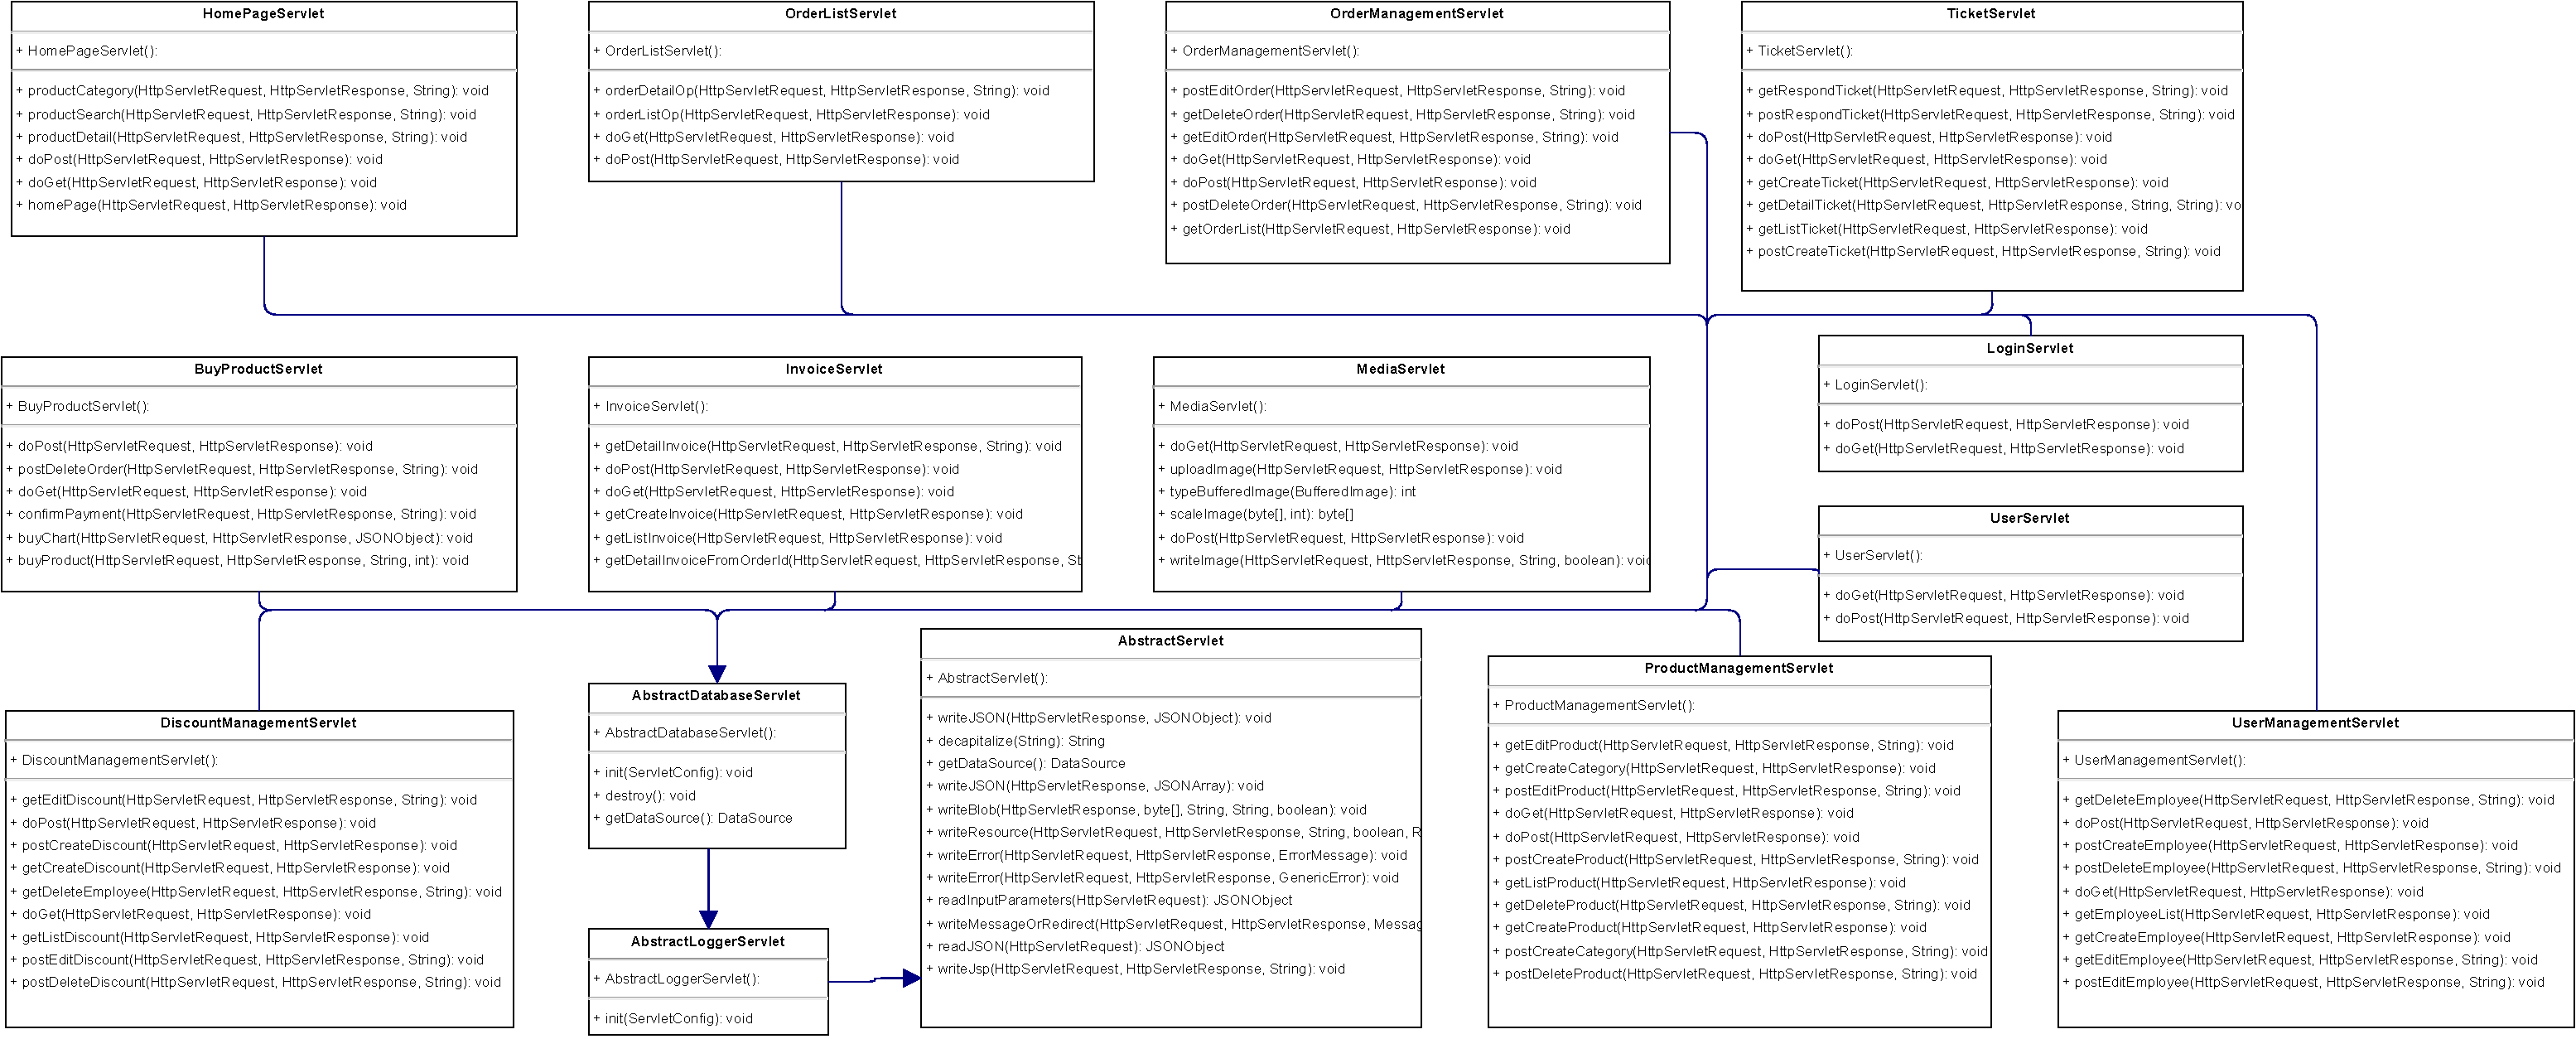
\includegraphics[width=\textwidth,height=\textheight,keepaspectratio]{Schemas/servlet.drawio.pdf}
    \caption{Servlet class diagram}
    \label{fig:ServletClassDiagram}
\end{figure}

\subsection*{Filter}

    
The filter package also contains an abstract class that takes care of 
initializing the common filter information, and the 4 classes that 
extend it take care of filtering the data by session.

In the figure \ref{fig:FilterClassDiagram} you can see the architecture 
of the filters. In the next pages we would use
the first letter of the filter class name to indicate the filter.
In particular \textbf{L} for \texttt{LoginFilter}, 
\textbf{A} for \texttt{AdminFilter}, \textbf{E} for 
\texttt{EmployeeFilter} and \textbf{C} for \texttt{CustomerFilter}.

A brief description of what the filters do:
\begin{itemize}
    \item \texttt{LoginFilter} check if the user is logged in
    \item \texttt{CustomerFilter} check if a customer is logged in
    \item \texttt{EmployeeFilter} check if an employee is logged in
    \item \texttt{AdminFilter} check if an administrator is logged in
\end{itemize}

\begin{figure}[H]
    \centering
    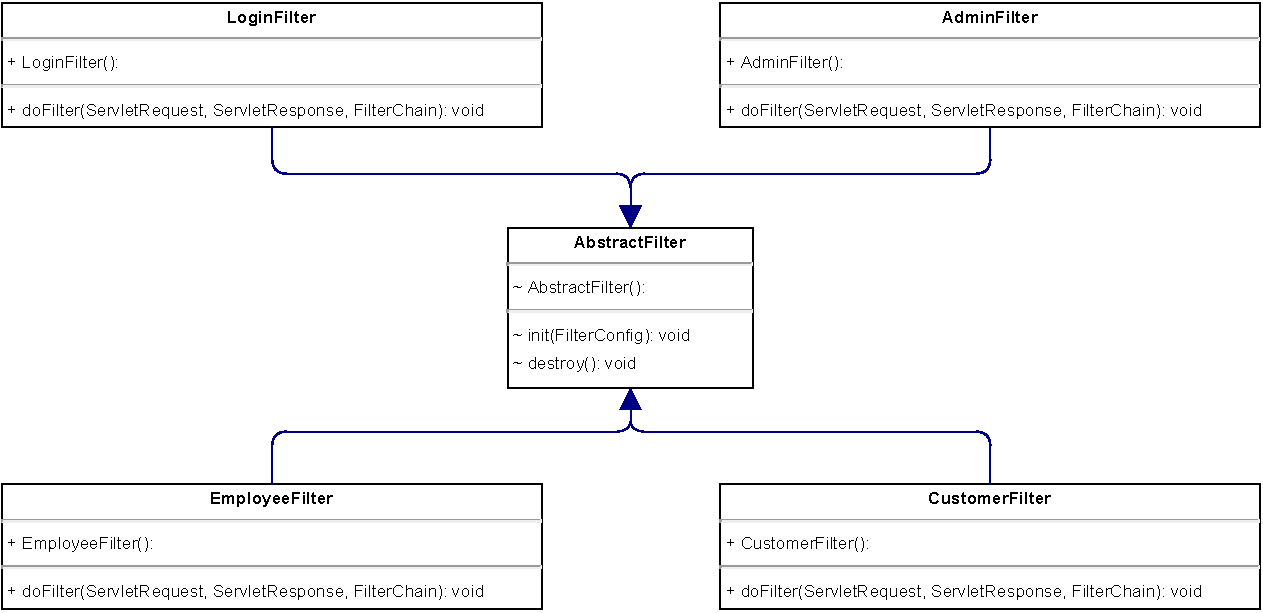
\includegraphics[width=0.7\textwidth]{Schemas/filter.drawio.pdf}
    \caption{Filter class diagram}
    \label{fig:FilterClassDiagram}
\end{figure}